\subsection{Estimação e Codificação Aritmética}

\begin{questions}
\question{
Suponha uma fonte i.i.d. com alfabeto $\mathcal{X} = \{a,b,c\}$.
Foi feita uma breve observação de símbolos produzidos por esta fonte
e observou-se 5 ocorrências do símbolo `a' e 2 ocorrências do símbolo `b'.
\begin{parts}
\part 
Utilize a regra de Laplace para estimar as probabilidades dos símbolos.
\part 
Explique qual é a razão de utilizarmos esta regra.
\part
Suponha a seguinte sequência de 2 símbolos $x_{1:2} = ab$. Qual
será a codificação binária dessa sequência dada pela codificação aritmética?
\end{parts}
}

\begin{solution}
\begin{parts} 
\part 
Temos que $N_a = 5$, $N_b = 2$ e $N_c = 0$.
Usando a regra de Laplace, teremos
\begin{eqnarray}
p(a) &=& \frac{5+1}{10} = \nicefrac{6}{10} \\
p(b) &=& \frac{2+1}{10} = \nicefrac{3}{10} \\
p(c) &=& \frac{0+1}{10} = \nicefrac{1}{10} 
\end{eqnarray}


\part 
Para que a estimativa da probabilidade de símbolos não observados não seja nula,
iremos adicionar 1 à frequência de ocorrência de todos os símbolos (regra de Laplace).
O fato de observamos um evento zero vezes ou uma única vez é apenas um acaso
decorrente da amostragem. Não devemos supor que um símbolo tenha probabilidade nula
pelo simples fato deste não ter ocorrido nenhuma vez em nossa amostra.
A regra de Laplace equivale a supor incerteza sobre os parâmetros da distribuição da fonte de forma
que os parâmetros possuam distribuição uniforme, o que levará à

\begin{equation}
p(s|x_{1:n}) = \frac{ N(s|x_{1:n}) + 1 }{\sum_{s'} (N(s'|x_{1:n}) + 1)}
\end{equation}



\part
 \

  %\begin{figure}[h!]
  %\centering
  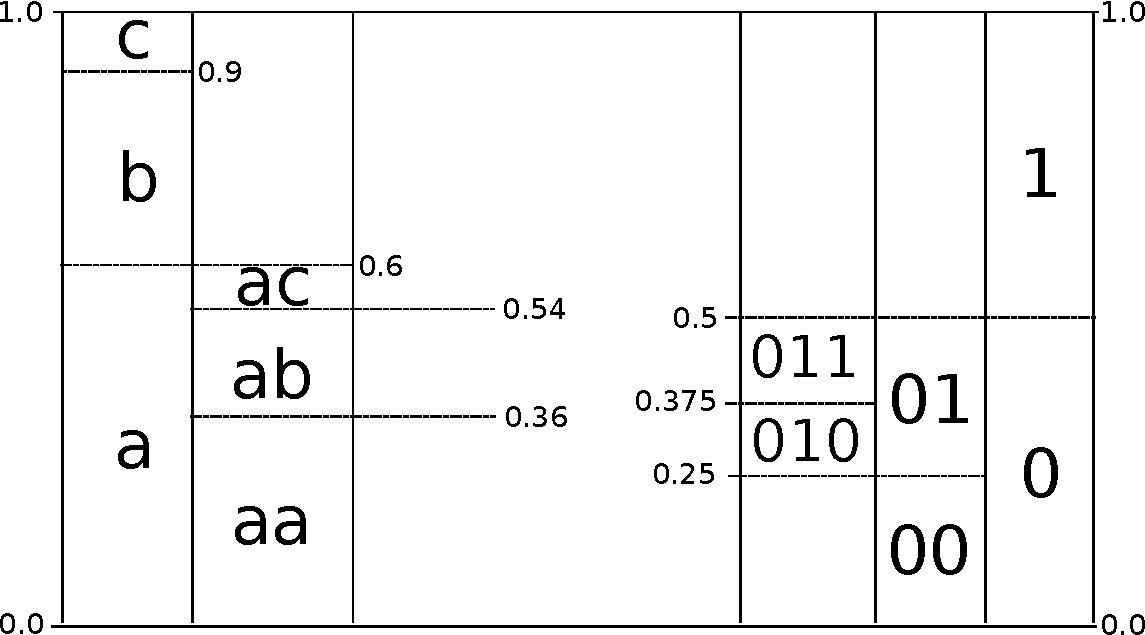
\includegraphics[width=0.8\textwidth]{../images/acoding.pdf}
  %\caption{Codificação Aritmética.}
  %\label{fig:acoding}
  %\end{figure}

\vspace{2em}
A sequência será codificada por 011 ou 100, dependendo da convenção.


\end{parts}
\end{solution}
\end{questions}
